
\bta{2010}


\section{Use of English}

\noindent
\textbf{Directions:}\\
Read the following text. Choose the best word (s) for each numbered
blank and mark A, B, C or D on \textbf{ANSWER
	SHEET 1}. (10 points)


\TiGanSpace


In 1924 America's National Research Council sent two engineers to
supervise a series of industrial experiments at a large telephone-parts
factory called the Hawthorne Plant near Chicago. It hoped they would
learn how shop-floor lighting \cloze workers' productivity.
Instead, the studies ended \cloze giving their name to the
``Hawthorne effect'', the extremely influential idea that the very
\cloze of being experimented upon changed subjects' behavior.

The idea arose because of the \cloze behavior of the women in the
Hawthorne plant. According to \cloze of the experiments, their
hourly output rose when lighting was increased, but also when it was
dimmed. It did not \cloze what was done in the experiment;
\cloze something was changed, productivity rose. A(n)
\cloze that they were being experimented upon seemed to be
\cloze to alter workers' behavior \cloze itself.

After several decades, the same data were \cloze to econometric
the analysis. The Hawthorne experiments has another surprise store.
\cloze the descriptions on record, no systematic \cloze
was found that levels of productivity were related to changes in
lighting.

It turns out that peculiar way of conducting the experiments may be have
let to \cloze interpretation of what happened. \cloze ,
lighting was always changed on a Sunday. When work started again on
Monday, output \cloze rose compared with the previous Saturday
and \cloze to rise for the next couple of days. \cloze ,
a comparison with data for weeks when there was no experimentation
showed that output always went up on Monday, Workers \cloze to
be diligent for the first few days of the week in any case, before
\cloze a plateau and then slackening off. This suggests that the
alleged ``Hawthorne effect'' is hard to pin down.


\newpage
\begin{enumerate}
	%\renewcommand{\labelenumi}{\arabic{enumi}.}
	% A(\Alph) a(\alph) I(\Roman) i(\roman) 1(\arabic)
	%设定全局标号series=example	%引用全局变量resume=example
	%[topsep=-0.3em,parsep=-0.3em,itemsep=-0.3em,partopsep=-0.3em]
	%可使用leftmargin调整列表环境左边的空白长度 [leftmargin=0em]
	\item


\fourchoices
{affected}
{achieved}
{extracted}
{restored}




\item


\fourchoices
{at}
{up}
{with}
{off}




\item


\fourchoices
{truth}
{sight}
{act}
{proof}




\item

\fourchoices
{controversial}
{perplexing}
{mischievous}
{ambiguous}


\item

\fourchoices
{requirements}
{explanations}
{accounts}
{assessments}



\item


\fourchoices
{conclude}
{matter}
{indicate}
{work}




\item

\fourchoices
{as far as}
{for fear that}
{in case that}
{so long so}



\item

\fourchoices
{awareness}
{expectation}
{sentiment}
{illusion}


\item


\fourchoices
{suitable}
{excessive}
{enough}
{abundant}




\item


\fourchoices
{about}
{for}
{on}
{by}




\item


\fourchoices
{compared}
{shown}
{subjected}
{conveyed}




\item

\fourchoices
{Contrary to}
{Consistent with}
{Parallel with}
{Peculiar to}



\item


\fourchoices
{evidence}
{guidance}
{implication}
{source}




\item

\fourchoices
{disputable}
{enlightening}
{reliable}
{misleading}



\item

\fourchoices
{In contrast}
{For example}
{In consequence}
{As usual}



\item

\fourchoices
{duly}
{accidentally}
{unpredictably}
{suddenly}



\item


\fourchoices
{failed}
{ceased}
{started}
{continued}




\item

\fourchoices
{Therefore}
{Furthermore}
{However}
{Meanwhile}



\item


\fourchoices
{attempted}
{tended}
{chose}
{intended}




\item


\fourchoices
{breaking}
{climbing}
{surpassing}
{hitting}

\end{enumerate}




\section{Reading Comprehension}



\noindent
\textbf{Part A}\\
\textbf{Directions:}\\
Read the following four texts. Answer the questions below each text by
choosing A, B, C or
D. Mark your answers on
\textbf{ANSWER SHEET 1}. (40 points)



\subsection{Text 1}


Of all the changes that have taken place in English-language newspapers
during the past quarter-century, perhaps the most far-reaching has been
the inexorable decline in the scope and seriousness of their arts
coverage.

It is difficult to the point of impossibility for the average reader
under the age of forty to imagine a time when high-quality arts
criticism could be found in most big-city newspapers. Yet a considerable
number of the most significant collections of criticism published in the
20th century consisted in large part of newspaper
reviews. To read such books today is to marvel at the fact that their
learned contents were once deemed suitable for publication in
general-circulation dailies.

We are even farther removed from the unfocused newspaper reviews
published in England between the turn of the 20th
century and the eve of World War II, at a time when newsprint was
dirt-cheap and stylish arts criticism was considered an ornament to the
publications in which it appeared. In those far-off days, it was taken
for granted that the critics of major papers would write in detail and
at length about the events they covered. Theirs was a serious business,
and even those reviewers who wore their learning lightly, like George
Bernard Shaw and Ernest Newman, could be trusted to know what they were
about. These men believed in journalism as a calling, and were proud to
be published in the daily press. ``So few authors have brains enough or
literary gift enough to keep their own end up in journalism,'' Newman
wrote, ``that I am tempted to define `journalism' as `a term of contempt
applied by writers who are not read to writers who are'.''

Unfortunately, these critics are virtually forgotten. Neville Cardus,
who wrote for the \emph{Manchester Guardian} from 1917 until shortly
before his death in 1975, is now known solely as a writer of essays on
the game of cricket. During his lifetime, though, he was also one of
England's foremost classical-music critics, a stylist so widely admired
that his \emph{Autobiography} (1947) became a best-seller. He was
knighted in 1967, the first music critic to be so honored. Yet only one
of his books is now in print, and his vast body of writings on music is
unknown save to specialists.

Is there any chance that Cardus's criticism will enjoy a revival? The
prospect seems remote. Journalistic tastes had changed long before his
death, and postmodern readers have little use for the richly upholstered
Vicwardian prose in which he specialized. Moreover, the amateur
tradition in music criticism has been in headlong retreat.


\begin{enumerate}[resume]
	%\renewcommand{\labelenumi}{\arabic{enumi}.}
	% A(\Alph) a(\alph) I(\Roman) i(\roman) 1(\arabic)
	%设定全局标号series=example	%引用全局变量resume=example
	%[topsep=-0.3em,parsep=-0.3em,itemsep=-0.3em,partopsep=-0.3em]
	%可使用leftmargin调整列表环境左边的空白长度 [leftmargin=0em]
	\item
It is indicated in Paragraphs 1 and 2 that \lineread.


\fourchoices
{arts criticism has disappeared from big-city newspapers}
{English-language newspapers used to carry more arts reviews}
{high-quality newspapers retain a large body of readers}
{young readers doubt the suitability of criticism on dailies}



\item
 Newspaper reviews in England before World War II were
characterized by \lineread.


\fourchoices
{free themes}
{casual style}
{elaborate layout}
{radical viewpoints}



\item
Which of the following would Shaw and Newman most probably
agree on?


\fourchoices
{It is writers' duty to fulfill journalistic goals.}
{It is contemptible for writers to be journalists.}
{Writers are likely to be tempted into journalism.}
{Not all writers are capable of journalistic writing.}



\item
 What can be learned about Cardus according to the last two
paragraphs?


\fourchoices
{His music criticism may not appeal to readers today.}
{His reputation as a music critic has long been in dispute.}
{His style caters largely to modern specialists.}
{His writings fail to follow the amateur tradition.}



\item
What would be the best title for the text?


\fourchoices
{Newspapers of the Good Old Days}
{The Lost Horizon in Newspapers}
{Mournful Decline of Journalism}
{Prominent Critics in Memory}

\end{enumerate}


\newpage
\subsection{Text 2}


Over the past decade, thousands of patents have been granted for what
are called business methods. Amazon.com received one for its  ``one-click''
online payment system. Merrill Lynch got legal protection for an asset
allocation strategy. One inventor patented a technique for lifting a
box.

Now the nation's top patent court appears completely ready to scale back
on business-method patents, which have been controversial ever since
they were first authorized 10 years ago. In a move that has
intellectual-property lawyers abuzz, the U.S. Court of Appeals for the Federal Circuit said
it would use a particular case to conduct a broad
review of business-method patents.  \emph{In re Bilski}, as the case is
known , is ``a very big deal'', says Dennis
D. Crouch of the University of
Missouri School of Law. It " has the potential to eliminate an entire
class of patents."

Curbs on business-method claims would be a dramatic \uline{about-face}, because
it was the Federal Circuit itself that introduced such patents with is
1998 decision in the so-called State Street Bank case, approving a
patent on a way of pooling mutual-fund assets. That ruling produced an
explosion in business-method patent filings, initially by emerging
Internet companies trying to stake out exclusive rights to specific
types of online transactions. Later, move established companies raced to
add such patents to their files, if only as a defensive move against
rivals that might beat them to the punch. In 2005, IBM noted in a court
filing that it had been issued more than 300 business-method patents,
despite the fact that it questioned the legal basis for granting them.
Similarly, some Wall Street investment films armed themselves with
patents for financial products, even as they took positions in court
cases opposing the practice.

The Bilski case involves a claimed patent on a method for hedging risk
in the energy market. The Federal Circuit issued an unusual order
stating that the case would be heard by all 12 of the court's judges,
rather than a typical panel of three, and that one issue it wants to
evaluate is whether it should ``reconsider'' its State Street Bank ruling.

The Federal Circuit's action comes in the wake of a series of recent
decisions by the Supreme Court that has narrowed the scope of
protections for patent holders. Last April, for example the justices
signaled that too many patents were being upheld for ``inventions'' that
are obvious. The judges on the Federal Circuit are ``reacting to the
anti-patent trend at the Supreme Court'', says Harold C. Wegner, a patent
attorney and professor at George Washington University Law School.


\begin{enumerate}[resume]
	%\renewcommand{\labelenumi}{\arabic{enumi}.}
	% A(\Alph) a(\alph) I(\Roman) i(\roman) 1(\arabic)
	%设定全局标号series=example	%引用全局变量resume=example
	%[topsep=-0.3em,parsep=-0.3em,itemsep=-0.3em,partopsep=-0.3em]
	%可使用leftmargin调整列表环境左边的空白长度 [leftmargin=0em]
	\item
Business-method patents have recently aroused concern
because of \lineread.

\fourchoices
{their limited value to business}
{their connection with asset allocation}
{the possible restriction on their granting}
{the controversy over authorization}



\item
Which of the following is true of the Bilski case?

\fourchoices
{Its ruling complies with the court decisions.}
{It involves a very big business transaction.}
{It has been dismissed by the Federal Circuit.}
{It may change the legal practices in the U.S.}


\item
The word ``about-face'' (Line 1, Para 3) most probably
means \lineread.
\fourchoices
{loss of good will}
{increase of hostility}
{change of attitude}
{enhancement of dignity}



\item
We learn from the last two paragraphs that business-method
patents \lineread.

\fourchoices
{are immune to legal challenges}
{are often unnecessarily issued}
{lower the esteem for patent holders}
{increase the incidence of risks}



\item
Which of the following would be the subject of the text?

\fourchoices
{A looming threat to business-method patents}
{Protection for business-method patent holders}
{A legal case regarding business-method patents}
{A prevailing trend against business-method patents}


\end{enumerate}


\newpage
\subsection{Text 3}


In his book \emph{The Tipping Point}, Malcolm Gladwell argues that ``social
epidemics'' are driven in large part by the acting of a tiny minority of
special individuals, often called influentials, who are unusually
informed, persuasive, or well-connected. The idea is intuitively
compelling, but it doesn't explain how ideas actually spread.

The supposed importance of influentials derives from a
plausible-sounding but largely untested theory called the " two-step
flow of communication": Information flows from the media to the
influentials and from them to everyone else. Marketers have embraced the
two-step flow because it suggests that if they can just find and
influence the influentials, those selected people will do most of the
work for them. The theory also seems to explain the sudden and
unexpected popularity of certain looks, brands, or neighborhoods. In
many such cases, a cursory search for causes finds that some small group
of people was wearing, promoting, or developing whatever it is before
anyone else paid attention. Anecdotal evidence of this kind fits nicely
with the idea that only certain special people can drive trends.

In their recent work, however, some researchers have come up with the
finding that influentials have far less impact on social epidemics than
is generally supposed. In fact, they don't seem to be required at all.

The researchers' argument stems from a simple observing about social
influence: With the exception of a few celebrities like Oprah
Winfrey---whose outsize presence is primarily a function of media, not
interpersonal, influence---even the most influential members of a
population simply don't interact with that many others. Yet it is
precisely these non-celebrity influentials who, according to the
two-step-flow theory, are supposed to drive social epidemics, by
influencing their friends and colleagues directly. For a social epidemic
to occur, however, each person so affected, must then influence his or
her own acquaintances, who must in turn influence theirs, and so on; and
just how many others pay attention to each of \uline{these people} has little to
do with the initial influential. If people in the network just two
degrees removed from the initial influential prove resistant, for
example, the cascade of change won't propagate very far or affect many
people.

Building on the basic truth about interpersonal influence, the
researchers studied the dynamics of social influence by conducting
thousands of computer simulations of populations, manipulating a number
of variables relating to people's ability to influence others and their
tendency to be influenced. They found that the principal requirement for
what is called ``global cascades''---the widespread propagation of
influence through networks---is the presence not of a few influentials
but, rather, of a critical mass of easily influenced people.


\begin{enumerate}[resume]
	%\renewcommand{\labelenumi}{\arabic{enumi}.}
	% A(\Alph) a(\alph) I(\Roman) i(\roman) 1(\arabic)
	%设定全局标号series=example	%引用全局变量resume=example
	%[topsep=-0.3em,parsep=-0.3em,itemsep=-0.3em,partopsep=-0.3em]
	%可使用leftmargin调整列表环境左边的空白长度 [leftmargin=0em]
	\item
By citing the book \emph{The Tipping Point}, the author
	intends to \lineread.


\fourchoices
{analyze the consequences of social epidemics}
{discuss influentials' function in spreading ideas}
{exemplify people's intuitive response to social epidemics}
{describe the essential characteristics of influentials}



\item
 The author suggests that the ``two-step-flow theory'' \lineread.


\fourchoices
{serves as a solution to marketing problems}
{has helped explain certain prevalent trends}
{has won support from influentials}
{requires solid evidence for its validity}


\item 
What the researchers have observed recently shows that \lineread.



\fourchoices
{the power of influence goes with social interactions}
{interpersonal links can be enhanced through the media}
{influentials have more channels to reach the public}
{most celebrities enjoy wide media attention}



\item
The underlined phrase ``these people'' in Paragraph 4 refers
to the ones who \lineread.


\fourchoices
{stay outside the network of social influence}
{have little contact with the source of influence}
{are influenced and then influence others}
{are influenced by the initial influential}


\item
 What is the essential element in the dynamics of social
influence?


\fourchoices
{The eagerness to be accepted.}
{The impulse to influence others.}
{The readiness to be influenced.}
{The inclination to rely on others.}

\end{enumerate}



\newpage
\subsection{Text 4}


Bankers have been blaming themselves for their troubles in public.
Behind the scenes, they have been taking aim at someone else: the
accounting standard-setters. Their rules, moan the banks, have forced
them to report enormous losses, and it's just not fair. These rules say
they must value some assets at the price a third party would pay, not
the price managers and regulators would like them to fetch.

Unfortunately, banks' lobbying now seems to be working. The details may
be unknowable, but the independence of standard-setters, essential to
the proper functioning of capital markets, is being compromised. And,
unless banks carry toxic assets at prices that attract buyers, reviving
the banking system will be difficult.

After a bruising encounter with Congress, America's Financial Accounting
Standards Board (FASB) rushed through rule changes. These gave banks
more freedom to use models to value illiquid assets and more flexibility
in recognizing losses on long-term assets in their income statement. Bob
Herz, the FASB's chairman, cried out against those who ``question our
motives.'' Yet bank shares rose and the changes enhance what one lobby
group politely calls ``the use of judgment by management.''

European ministers instantly demanded that the International Accounting
Standards Board (IASB) do likewise. The IASB says it does not want to
act without overall planning, but the pressure to fold when it completes
it reconstruction of rules later this year is strong. Charlie McCreevy,
a European commissioner, warned the IASB that it did ``not live in a
political vacuum'' but ``'in the real word'' and that Europe could yet
develop different rules.

It was banks that were \uline{on the wrong planet}, with accounts that vastly
overvalued assets. Today they argue that market prices overstate losses,
because they largely reflect the temporary illiquidity of markets, not
the likely extent of bad debts. The truth will not be known for years.
But bank's shares trade below their book value, suggesting that
investors are skeptical. And dead markets partly reflect the paralysis
of banks which will not sell assets for fear of booking losses, yet are
reluctant to buy all those supposed bargains.

To get the system working again, losses must be recognized and dealt
with. America's new plan to buy up toxic assets will not work unless
banks mark assets to levels which buyers find attractive. Successful
markets require independent and even combative standard-setters. The
FASB and IASB have been exactly that, cleaning up rules on stock options
and pensions, for example, against hostility from special interests. But
by giving in to critics now they are inviting pressure to make more
concessions.

\begin{enumerate}[resume]
	%\renewcommand{\labelenumi}{\arabic{enumi}.}
	% A(\Alph) a(\alph) I(\Roman) i(\roman) 1(\arabic)
	%设定全局标号series=example	%引用全局变量resume=example
	%[topsep=-0.3em,parsep=-0.3em,itemsep=-0.3em,partopsep=-0.3em]
	%可使用leftmargin调整列表环境左边的空白长度 [leftmargin=0em]
	\item
Bankers complained that they were forced to \lineread.


\fourchoices
{follow unfavorable asset evaluation rules}
{collect payments from third parties}
{cooperate with the price managers}
{re-evaluate some of their assets}



\item
According to the author, the rule changes of the FASB may
result in \lineread.


\fourchoices
{the diminishing role of management}
{the revival of the banking system}
{the banks' long-term asset losses}
{the weakening of its independence}


\item
According to Paragraph 4, McCreevy objects to the IASB's
attempt to \lineread.


\fourchoices
{keep away from political influences}
{evade the pressure from their peers}
{act on their own in rule-setting}
{take gradual measures in reform}



\item
The author thinks the banks were ``on the wrong planet'' in
that they \lineread.


\fourchoices
{misinterpreted market price indicators}
{exaggerated the real value of their assets}
{neglected the likely existence of bad debts}
{denied booking losses in their sale of assets}



\item
The author's attitude towards standard-setters is one of \lineread.


\fourchoices
{satisfaction}
{skepticism}
{objectiveness}
{sympathy}


\end{enumerate}


\newpage

\noindent
\textbf{Part B}\\
\textbf{Directions:}\\
For Questions 41-45, choose the most suitable paragraphs from the list
A-G and fill them into the numbered boxes to form a coherent text.
Paragraph E has been correctly placed. There is one paragraph which does
not fit in with the text. Mark your answers on \textbf{ANSWER SHEET 1}.
(10 points)

\begin{listmatch}
	%\renewcommand{\labelenumi}{\arabic{enumi}.}
	% A(\Alph) a(\alph) I(\Roman) i(\roman) 1(\arabic)
	%设定全局标号series=example	%引用全局变量resume=example
	%[topsep=-0.3em,parsep=-0.3em,itemsep=-0.3em,partopsep=-0.3em]
	%可使用leftmargin调整列表环境左边的空白长度 [leftmargin=0em]
	\item
The first and more important is the consumer's growing
preference for eating out: the consumption of food and drink in places
other than homes has risen from about 32 percent of total consumption in
1995 to 35 percent in 2000 and is expected to approach 38 percent by
2005. This development is boosting wholesale demand from the food
service segment by 4 to 5 percent a year across Europe, compared with
growth in retail demand of 1 to 2 percent. Meanwhile, as the recession
is looming large, people are getting anxious. They tend to keep a
tighter hold on their purse and consider eating at home a realistic
alternative.


\item 
 Retail sales of food and drink in Europe's largest markets are
at a standstill, leaving European grocery retailers hungry for
opportunities to grow. Most leading retailers have already tried
e-commerce, with limited success, and expansion abroad. But almost all
have ignored the big, profitable opportunity in their own backyard: the
wholesale food and drink trade, which appears to be just the kind of
market retailers need.


\item 
 Will such variations bring about a change in the overall
structure of the food and drink market? Definitely not. The functioning
of the market is based on flexible trends dominated by potential buyers.
In other words, it is up to the buyer, rather than the seller, to decide
what to buy. At any rate, this change will ultimately be acclaimed by an
ever-growing number of both domestic and international consumers,
regardless of how long the current consumer pattern will take hold.


\item 
 All in all, this clearly seems to be a market in which big
retailers could profitably apply their gigantic scale, existing infrastructure
and proven skills in the management of product ranges, logistics, and
marketing intelligence. Retailers that master the intricacies of
wholesaling in Europe may well expect to rake in substantial profits
thereby. At least, that is how it looks as a whole. Closer inspection
reveals important differences among the biggest national markets,
especially in their customer segments and wholesale structures, as well
as the competitive dynamics of individual food and drink categories. Big
retailers must understand these differences before they can identify the
segments of European wholesaling in which their particular abilities
might unseat smaller but entrenched competitors. New skills and
unfamiliar business models are needed too.


\item 
 Despite variations in detail, wholesale markets in the countries
that have been closely examined---France, Germany, Italy, and
Spain---are made out of the same building blocks. Demand comes mainly
from two sources: independent mom-and-pop grocery stores which, unlike
large retail chains, are too small to buy straight from producers, and
food service operators that cater to consumers when they don't eat at
home. Such food service operators range from snack machines to large
institutional catering ventures, but most of these businesses are known
in the trade as ``horeca'': hotels, restaurants, and cafes. Overall,
Europe's wholesale market for food and drink is growing at the same
sluggish pace as the retail market, but the figures, when added
together, mask two opposing trends.


\item 
 For example, wholesale food and drink sales come to \$268
billion in France, Germany, Italy, Spain, and the United Kingdom in
2000---more than 40 percent of retail sales. Moreover, average overall
margins are higher in wholesale than in retail; wholesale demand from
the food service sector is growing quickly as more Europeans eat out
more often; and changes in the competitive dynamics of this fragmented
industry are at last making it feasible for wholesalers to consolidate.


\item 
 However, none of these requirements should deter large retailers
(and even some large food producers and existing wholesalers) from
trying their hand, for those that master the intricacies of wholesaling
in Europe stand to reap considerable gains.
\end{listmatch}


\[ 
\begin{tabular}{|c|c|}
	\hline
	41. &  \hspace{1.5em} \\
	\hline
\end{tabular}
\rightarrow
\begin{tabular}{|c|c|}
	\hline
	42. &  \hspace{1.5em} \\
	\hline
\end{tabular}
\rightarrow
\begin{tabular}{|c|c|}
	\hline
	43. &  \hspace{1.5em} \\
	\hline
\end{tabular}
\rightarrow
\begin{tabular}{|c|c|}
	\hline
	44. &  \hspace{1.5em} \\
	\hline
\end{tabular}
\rightarrow
\begin{tabular}{|c|}
	\hline
	E \\
	\hline
\end{tabular}
\rightarrow
\begin{tabular}{|c|c|}
	\hline
	45. &  \hspace{1.5em} \\
	\hline
\end{tabular}
 \]


\phantom{ \linefill \linefill \linefill \linefill \linefill}


\newpage
\noindent
\textbf{Part C}\\
\textbf{Directions:}\\
Read the following text carefully and then translate the underlined
segments into Chinese. Your translation should be written carefully on
\textbf{ANSWER SHEET 2}. (10 points)



\TiGanSpace


One basic weakness in a conservation system based wholly on economic
motives is that most members of the land community have no economic
value. Yet these creatures are members of the biotic community and, if
its stability depends on its integrity, they are entitled to
continuance.

When one of these noneconomic categories is threatened and, if we happen
to love it. We invert excuses to give it economic importance. At the
beginning of century songbirds were supposed to be disappearing.  \transnum 
\uline{Scientists jumped to the rescue with some distinctly shaky
	evidence to the effect that insects would eat us up if birds failed to
	control them.} the evidence had to be economic in order to be valid.

It is painful to read these round about accounts today. We have no land
ethic yet, \transnum \uline{but we have at least drawn near the point of
	admitting that birds should continue as a matter of intrinsic right,
	regardless of the presence or absence of economic advantage to us.}

A parallel situation exists in respect of predatory mammals and
fish-eating birds. \transnum \uline{Time was when biologists somewhat
	overworked the evidence that these creatures preserve the health of
	game by killing the physically weak, or that they prey only on
	``worthless'' species.}

Some species of tree have been read out of the party by economics-minded
foresters because they grow too slowly, or have too low a sale vale to
pay as timber crops. \transnum \uline{In Europe, where forestry is
	ecologically more advanced, the non-commercial tree species are
	recognized as members of native forest community, to be preserved as
	such, within reason.}

To sum up: a system of conservation based solely on economic
self-interest is hopelessly lopsided. \transnum \uline{It tends to
	ignore, and thus eventually to eliminate, many elements in the land
	community that lack commercial value, but that are essential to its
	healthy functioning.} It assumes, falsely, I think, that the economic
parts of the biotic clock will function without the uneconomic parts.



\section{Writing}


\noindent
\textbf{Part A}\\
\textbf{51. Directions:}




You are supposed to write for the postgraduate association a notice to
recruit volunteers for an international conference on globalization, you
should conclude the basic qualification of applicant and the other
information you think relative.

You should write about 100 words on \textbf{ANSHWER SHEET 2}.

 \textbf{Do not} sign your own name at
the end of the letter. Use ``postgraduate association'' instead. (10 points)



\vspace{2em}

\noindent
\textbf{Part B}\\
\textbf{52. Directions:}

Write an essay of 160-200 words based on the following drawing. In your
essay, you should
\begin{listwrite}
	%\renewcommand{\labelenumi}{\arabic{enumi}.}
	% A(\Alph) a(\alph) I(\Roman) i(\roman) 1(\arabic)
	%设定全局标号series=example	%引用全局变量resume=example
	%[topsep=-0.3em,parsep=-0.3em,itemsep=-0.3em,partopsep=-0.3em]
	%可使用leftmargin调整列表环境左边的空白长度 [leftmargin=0em]
	\item
 describe the drawing briefly,

\item 
 explain its intended meaning, and 

\item 
 give your comments.
\end{listwrite}

You should write neatly on \textbf{ANSHWER SHEET 2}. (20 points)


\begin{figure}[h!]
	\centering
	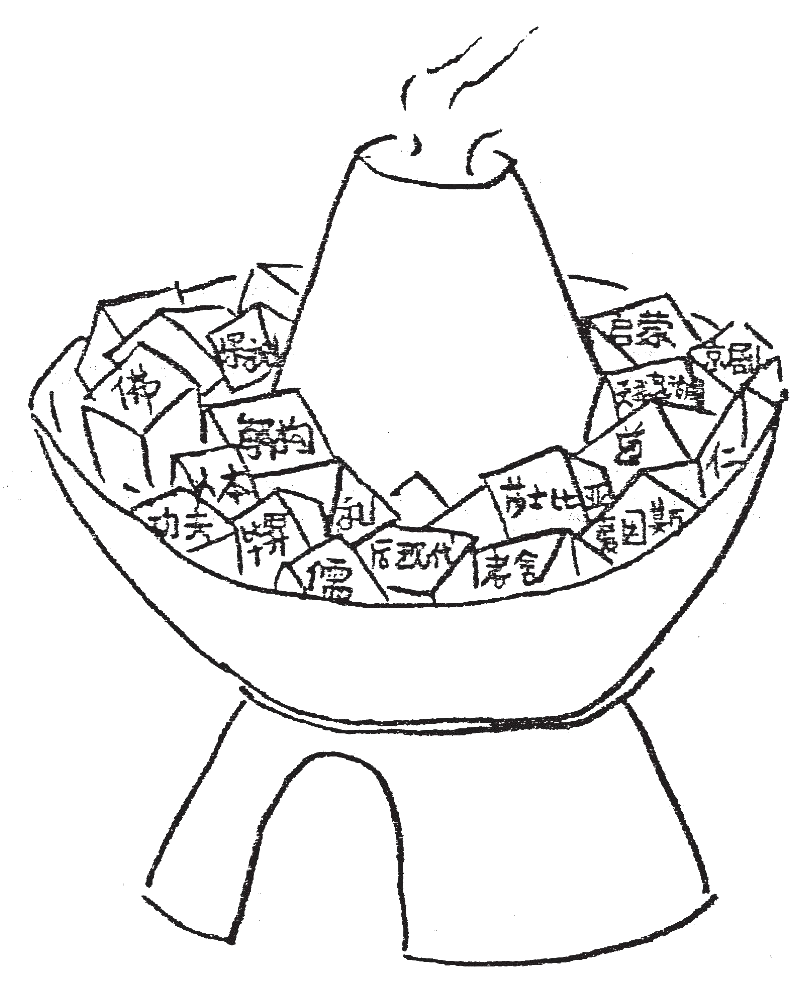
\includegraphics[width=0.36\linewidth]{picture/2010.png}
	\caption*{文化“火锅”,既美味又营养}
\end{figure}

